\documentclass{beamer}
\usetheme{Berkeley}
\usepackage{graphicx}

\begin{document}

%no errors, but jitter
% \begin{frame}
% \begin{tabular}{ccc}
% \only<1-7>{
\includegraphics[width=0.3\linewidth]{1}&}
% \only<2-7>{
\includegraphics[width=0.3\linewidth]{2}&}
% \only<3-7>{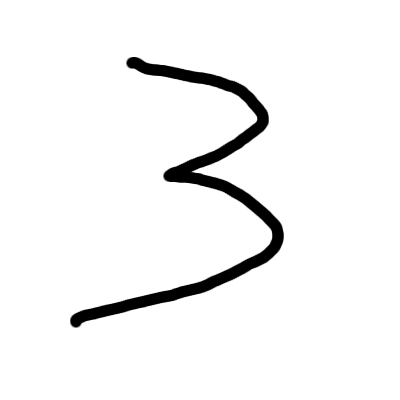
\includegraphics[width=0.3\linewidth]{3}\\}
% \only<4-7>{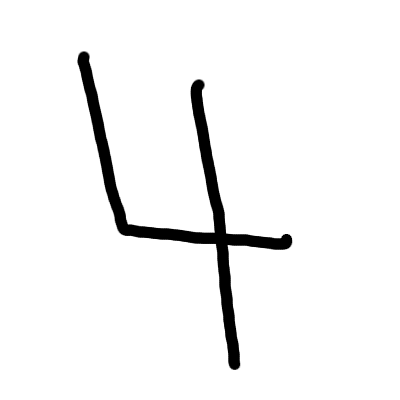
\includegraphics[width=0.3\linewidth]{4}&}
% \only<5>{
\includegraphics[width=0.3\linewidth]{5}&}
% \only<6-7>{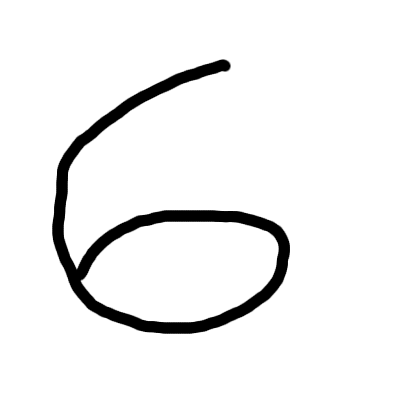
\includegraphics[width=0.3\linewidth]{6}&}
% \only<7>{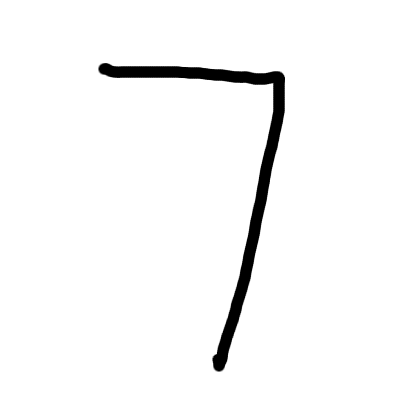
\includegraphics[width=0.3\linewidth]{7}}
% \end{tabular}
% \end{frame}

%errors
% \begin{frame}
% \begin{tabular}{ccc}
% \uncover<1-7>{
\includegraphics[width=0.3\linewidth]{1}&}
% \uncover<2-7>{
\includegraphics[width=0.3\linewidth]{2}&}
% \uncover<3-7>{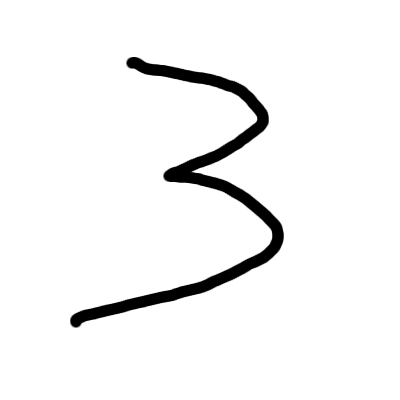
\includegraphics[width=0.3\linewidth]{3}\\}
% \uncover<4-7>{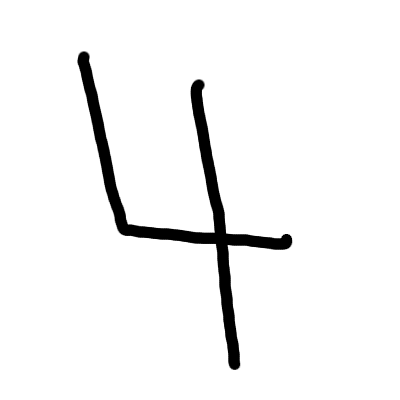
\includegraphics[width=0.3\linewidth]{4}&}
% \only<5>{
\includegraphics[width=0.3\linewidth]{5}&}
% \uncover<6-7>{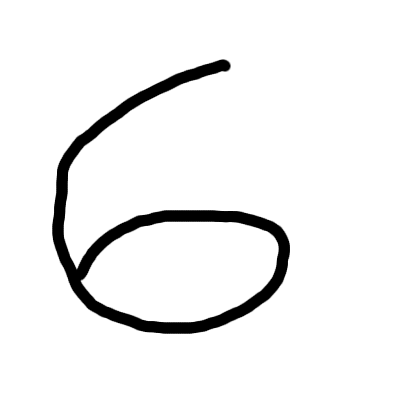
\includegraphics[width=0.3\linewidth]{6}&}
% \uncover<7>{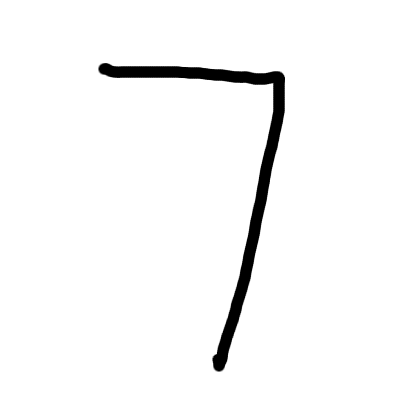
\includegraphics[width=0.3\linewidth]{7}}
% \end{tabular}
% \end{frame}

\begin{frame}
\begin{tabular}{ccc}
\only<1-7>{
\begin{figure}[!ht]
\fbox{\rule{0pt}{2in} \rule{0.3\linewidth}{0pt}}
\end{figure} &
}
\only<2-7>{
\begin{figure}[!ht]
\fbox{\rule{0pt}{2in} \rule{0.3\linewidth}{0pt}}
\end{figure} &
}
\only<3-7>{
\begin{figure}[!ht]
\fbox{\rule{0pt}{2in} \rule{0.3\linewidth}{0pt}}
\end{figure} \\
}
\only<4-7>{
\begin{figure}[!ht]
\fbox{\rule{0pt}{2in} \rule{0.3\linewidth}{0pt}}
\end{figure} &
}
\only<5>{
\begin{figure}[!ht]
\fbox{\rule{0pt}{2in} \rule{0.3\linewidth}{0pt}}
\end{figure} &
}
\only<6-7>{
\begin{figure}[!ht]
\fbox{\rule{0pt}{2in} \rule{0.3\linewidth}{0pt}}
\end{figure} &
}
\only<7>{
\begin{figure}[!ht]
\fbox{\rule{0pt}{2in} \rule{0.3\linewidth}{0pt}}
\end{figure} 
}
\end{tabular}
\end{frame}

\end{document} 